%%%%%%%%%%%%%%%%%%%%%%%%%%%%%%%%%%%%%
%%%%%%%%%%%%%%%%%%%%%%%%%%%%%%%%%%%%%
%
%   Hi, All 
%
%   Arun Xavier, 
%   Subscribe, Comment at Youtube Channel 
%
%   https://www.youtube.com/c/arunxaviertech
%
%
%   for more  Visit my Page - http://arunxeee.blogspot.in/
%
%%%%%%%%%%%%%%%%%%%%%%%%%%%%%%%%%%%%
%%%%%%%%%%%%%%%%%%%%%%%%%%%%%%%%%%%%
\documentclass[12 pt, oneside]{book}
%%%%%%%%%%%%%%%%%%%%%%%%%%%%%%%%%%%%%
%%%%%%%%%%%%%%%%%%%%%%%%%%%%%%%%%%%%%
%
%   Hi, All 
%
%   Arun Xavier, 
%   Subscribe, Comment at Youtube Channel 
%
%   https://www.youtube.com/c/arunxaviertech
%
%
%   for more  Visit my Page - http://arunxeee.blogspot.in/
%
%%%%%%%%%%%%%%%%%%%%%%%%%%%%%%%%%%%%
%%%%%%%%%%%%%%%%%%%%%%%%%%%%%%%%%%%%

\usepackage{graphicx, fancyhdr, amsmath, times, enumerate,geometry,makeidx,setspace,nomencl,eso-pic,xcolor,lipsum,calc,pst-node,tikz,fancybox,background,caption,subcaption,amsfonts}




\usetikzlibrary{calc}
\SetBgScale{1}
\SetBgAngle{0}
\SetBgColor{brown}
\SetBgOpacity{1}
%%
\geometry{verbose,a4paper,tmargin=1 in,bmargin=1in,lmargin=1.5 in,rmargin=.9 in}
%%%%%%%%%%%%%%%%%%%%%%%%%%%%%%%

\makeindex

%%
\usepackage[final]{pdfpages}
%%
%\setlength{\oddsidemargin}{2 cm}



%%
\newcommand{\VAtitle}[1]%
{\def\vtitle{#1}}%
\newcommand{\VAauthor}[1]%
{\def\vauthor{#1}}%
\newcommand{\VAauthora}[1]%
{\def\vauthora{#1}}%
\newcommand{\VAauthorb}[1]%
{\def\vauthorb{#1}}%
\newcommand{\VAauthorc}[1]%
{\def\vauthorc{#1}}%
\newcommand{\VAauthord}[1]%
{\def\vauthord{#1}}%
\newcommand{\VAadmissionyear}[1]%
{\def\vadmissionyear{#1}}%
\newcommand{\VAacademicyear}[1]%
{\def\vacademicyear{#1}}%
\newcommand{\VAregisternumber}[1]%
{\def\vregisternumber{#1}}%
\newcommand{\VAprincipal}[1]%
{\def\vprincipal{#1}}%
\newcommand{\VAguide}[1]%
{\def\vguide{#1}}%
\newcommand{\VAguidedg}[1]%
{\def\vguidedg{#1}}%
\newcommand{\VAcoguide}[1]%
{\def\vcoguide{#1}}%
\newcommand{\VAcoguidedg}[1]%
{\def\vcoguidedg{#1}}%
\newcommand{\VAhod}[1]%
{\def\vhod{#1}}%
\newcommand{\VAdate}[1]%
{\def\vdate{#1}}%
\newcommand{\VAdept}[1]%
{\def\vdept{#1}}%
\newcommand{\VAclass}[1]%
{\def\vclass{#1}}%
\newcommand{\VApaper}[1]%
{\def\vpaper{#1}}%
\newcommand{\VAdeptst}[1]%
{\def\vdeptst{#1}}%

%%
%%



\SetBgContents{}



\VApaper{PROJECT PRELIMINARY REPORT}

\usepackage{titlesec}
\titleformat{\chapter}[display]
{\normalfont\LARGE\bfseries\centering}{\chaptertitlename\ \thechapter}{20pt}{\Huge}

\begin{document}
%%%%%%%%%%%%%%%%%%%%%%%%%%%%%%%%%%%%
%%%%%%%%%%%%%%%%%%%%%%%%%%%%%%%%%%%%
%%
%%          Edit the Names & others from below onwards. . .
%%
%%%%%%%%%%%%%%%%%%%%%%%%%%%%%%%%%%%%
%%%%%%%%%%%%%%%%%%%%%%%%%%%%%%%%%%%%

\VAtitle{MAIN PROJECT TITLE}

%%%%%%%%%%%%%%%%%%%%%%%%%%%%%%
%   
%	Give Students name in Alphabetical Order 
%
%%%%%%%%%%%%%%%%%%%%%%%%%%%%%%
\VAauthora{STD Name 1 (VAS21000)}
\VAauthorb{STD Name 2 (VAS21000)}
\VAauthorc{STD Name 3 (VAS21000)}
\VAauthord{STD Name 4 (VAS21000)}

%%%%%%%%%%%%%%%%%%%%%%%%%%%%%%%%
%
%	Give details of Main Author, (to be seen in the certificate, etc.)
%
%%%%%%%%%%%%%%%%%%%%%%%%%%%%%%%%
%
%   In the next line, replace "Student" by your name. 
%   Write full name without, Mr. or Ms.
%
\VAauthor{STUDENT NAME} % all students name with ","
\VAadmissionyear{2023}
%   University Examination Register Number.
%
\VAregisternumber{VAS23EE000} % all students uni no. with ","
%
%%%%%%%%%%%%%%%%%%%%%%%%%%%%%%%%
%
\VAacademicyear{2026-2027}%
%   the full name of your principal
%
\VAprincipal{Dr Sunitha C.}
%   In the next line, replace "HoD" by the full name of Head of Department with Mr. or Ms. or Dr. or Prof.
%
\VAhod{Dr Vinila M. L.}
%
%  the full name of your guide or supervisor 
\VAguide{Guides Name}% 
\VAguidedg{Asst. Prof.,} % Give your Guides Designation Asst. Prof., Asso. Prof.
\VAcoguide{Co-guides Name}% 
\VAcoguidedg{Asst. Prof.,} % Give your Co-guides Designation Asst. Prof., Asso. Prof.

%   Enter the Sem End month like "December"
%   Type Month and Year
\VAdate{December 2026}%
\VAdept{Electrical and Electronics}%
% dept in Shot Eg: EEE, ME
\VAdeptst{EEE}
\VAclass{Seventh Semester B.Tech}%
%%%%%%%%%%%%%%%%%%%%%%%%%%%%%%%%%%%%%

%%%%%%%%%%%%%%%%%%%%%%%%%%%%%%%%%%%%
%%%%%%%%%%%%%%%%%%%%%%%%%%%%%%%%%%%%
\input{frontmatter}
%%%%%%%%%%%%%%%%%%%%%%%%%%%%%%%%%%%%
%%%%%%%%%%%%%%%%%%%%%%%%%%%%%%%%%%%%

\chapter*{\centering{Abstract}}
\addcontentsline{toc}{chapter}{\quad ABSTRACT}

Copy Paste Your Abstract here . . . 


%%%%%%%%%%%%%%%%%%%%%%%%%%%%%%%%%%%%
%%%%%%%%%%%%%%%%%%%%%%%%%%%%%%%%%%%%
%       
%		Do not change any thing after this . . .
%
%%%%%%%%%%%%%%%%%%%%%%%%%%%%%%%%%%%%
%%%%%%%%%%%%%%%%%%%%%%%%%%%%%%%%%%%%
\tableofcontents
\addcontentsline{toc}{chapter}{\quad  LIST OF FIGURES}
\listoffigures
\addcontentsline{toc}{chapter}{\quad  LIST OF TABLES}
\listoftables
% For adding List of symbols or abbreviations
\addcontentsline{toc}{chapter}{\quad  LIST OF SYMBOLS AND ABBREVIATIONS}
%%%%%%%%%%%%%%%%%%%%%%%%%%%%%%%%%%%%%
%%%%%%%%%%%%%%%%%%%%%%%%%%%%%%%%%%%%%
%
%   Hi, All 
%
%   Arun Xavier, 
%   Subscribe, Comment at Youtube Channel 
%
%   https://www.youtube.com/c/arunxaviertech
%
%
%   for more  Visit my Page - http://arunxeee.blogspot.in/
%
%%%%%%%%%%%%%%%%%%%%%%%%%%%%%%%%%%%%
%%%%%%%%%%%%%%%%%%%%%%%%%%%%%%%%%%%%


\chapter*{List of Symbols and Abbreviations}


%% Write in alphabetical order
%% Write in alphabetical order
%% Write in alphabetical order
%% Write in alphabetical order


\begin{tabbing}



\hspace{1cm}\= {$ \bf ABCD  $}\qquad\ \quad\= Use in alphabetical order\\[5pt]

\> {$ \bf A_i  $} \> Area of the $i^{th}$ component\\[5pt]

\> {$ \bf DC $} \>   Direct current electricity\\[5pt]

\> {$ \bf DSO  $} \> Digital Storage Oscilloscope\\[5pt]

\> {$ \bf FBI  $} \> Full Bridge Inverter\\



\end{tabbing}
\mainmatter
%%%%%%%%%%%%%%%%%%%%%%%%%%%%%%%%%%%%%
%%%%%%%%%%%%%%%%%%%%%%%%%%%%%%%%%%%%%
%%    
%%    Copy your Project Work below from Here
%%
%%%%%%%%%%%%%%%%%%%%%%%%%%%%%%%%%%%%%
%%%%%%%%%%%%%%%%%%%%%%%%%%%%%%%%%%%%%



\chapter{INTRODUCTION}

{\em Give some intro about this chapter . . .. .  . 

Electrical engineering is a field of engineering that generally deals with the study and application of electricity, electronics, and electromagnetism. This field first became an identifiable occupation in the latter half of the 19th century after commercialization of the electric telegraph, the telephone, and electric power distribution and use.\cite{a} Photovoltaic (PV) \index{Photovoltaic}power supplied to the system is gaining more and more visibility. \cite{b}

Photovoltaic (PV) power supplied to the system is gaining more and more visibility Solid-state inverters have shown for the enabling technology for putting PV systems now. \cite{b} }


% You can add any sections like that . . . 

\section{Objectives of the Work}


\begin{figure}[h]
\centering
\label{fig}
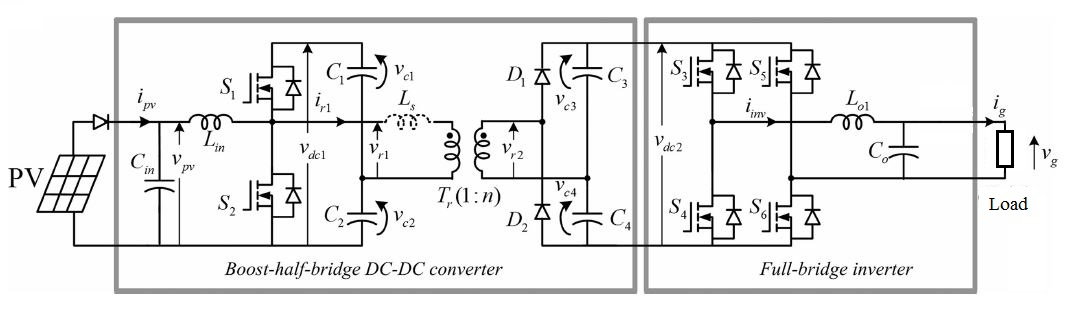
\includegraphics[width= 14 cm]{ct.jpg}
\caption{ Circuit Diagram}
\end{figure}

The concept of micro-inverter (also known as a module integrated converter / inverter) has become a future trend for single phase  photovoltaic (PV) power. In general, a micro-inverter PV \index{Photovoltaic} is often provided by a low voltage solar panel, which requires a high voltage lift ratio to the Fig: 1.1 produce the desired AC output .  %\ref for the figure label, check the below figure.

%%%%%%%%%%%%%%%%%%%%%%%%%%%%%%%%%%%
%		Before using image put the jpg image file in the folder. 
%		Here   ct.jpg   is the file name
%%%%%%%%%%%%%%%%%%%%%%%%%%%%%%%%%%%



\section{Motivation for this work}

There are  . . .

\section{Methodologies Adopted}

Methodologies adopted for this project . . . .


\section{Outline of the Report}

This report contains 6 chapters. Chapter 1 gives the introduction to the project work and describes the objectives of the work. Literature survey is describes in Chapter 2. An introduction to the pro............

\section{Summary}

{\em Give summary abt this chapter \& brief into about the next Chapter.}

\chapter{LITERATURE REVIEW}


{\em Give some intro abt this chapter . . .. .  . }


\section{Paper I \cite{a}}
Details about paper one. Here you write abt the details in the IEEE paper(Intro + Conclusion) or about the work who had done before, what are the problems at that time, etc.

\section{Paper II\cite{b}}
Details about paper two. Here you write abt the details in the IEEE paper(Intro + Conclusion) or about the work who had done before, what are the problems at that time, etc


\section{Paper III\cite{c}}
Details about paper three. Here you write abt the details in the IEEE paper(Intro + Conclusion) or about the work who had done before, what are the problems at that time, etc


\section{Paper IV}
Details about paper four. Here you write abt the details in the IEEE paper(Intro + Conclusion) or about the work who had done before, what are the problems at that time, etc

\begin{enumerate}
    \item Paper I
    \item Paper II
\end{enumerate}

To use bullets

\begin{itemize}
\item{Presented}
\item{Paper}
\item{Presented}
\item{Paper}
\end{itemize}

General, a micro-inverter PV \index{Photovoltaic} is often provided by a low voltage solar panel, which requires a high voltage lift ratio to produce the desired AC output .


\begin{itemize}
\item{Presented}
\item{Paper  }
	\begin{itemize}
		\item{Presented}
		\item{Paper  }
	\end{itemize}
\item{Presented}
\item{Paper  }
\end{itemize}


Inverter has become a future trend for single phase photovoltaic (PV) power. In general, a micro-inverter PV \index{Photovoltaic} is often provided by a low voltage solar panel . . . \vspace{2 cm} % Vspace to leave 2 cm space




To use 1,2,3, numbers

\begin{enumerate}
\item prepare a source file with the extension "tex"
\item Compile it with \LaTeX to produce a "dvi" file
\item Print the document using a "dvi" driver
\end{enumerate}


For making a table . .. .

\begin{table}[h]
\centering
\begin{tabular}{|l|r|}  % use c for center alignment
\hline \hline
Planet & Diameter(km)\\
\hline \hline
Mercury & 4878\\
Pluto & 2274\\
Mercury & 4878\\
Pluto & 2274\\
Mercury & 4878\\
Pluto & 2274\\
Mercury & 4878\\
Pluto & 2274\\
\hline
\end{tabular}
\caption{Table Name}
\end{table}


$$
ax+by+c=0
$$


\section{Summary}

{\em Give summary abt this chapter \& brief into about the next Chapter.}








\chapter{METHODOLOGIES FOR THE PROJECT}  % Short of the project name

{\em Give some intro abt this chapter . . .. .  . }


\section{Block Diagram}

Explain different stages in the block diagram with figure . . .




\section{Circuit Diagram}

\begin{figure}[h]
\label{sss}
\centering
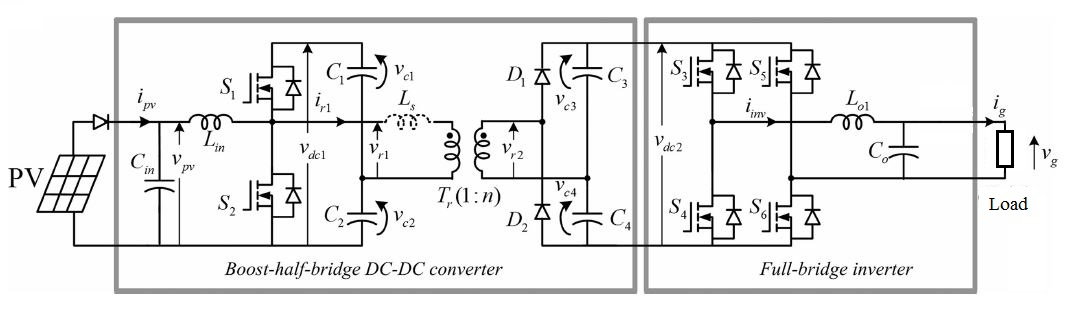
\includegraphics[width= 14 cm]{ct.jpg}
\caption{ Circuit Diagram}
\end{figure}

Explain different stages in the circuit diagram with figure . . .

For equ..

\begin{equation}
d_fT_s=i_{pk}/m_2=i_{pk}L_1/(V_0-v_{ik})
\end{equation}

During this switching cycle, the energy ($E_k$) transferred
from the input to the output can be obtained as:

\begin{equation}
E_k=v_{ik}.i_{pk}.T_s(D+d_f)/2
\end{equation}

\section{Control Part}

Explain different stages in the control part PIC, 8085, etc . . . 

\section{Power Circuit Part}

The duty cycle of S1 is denoted by d1. The switching period of the pulse half-bridge converter is $T_{sw1}$. PV current and voltage are represented by $I_{PV}$ and $V_{PV},$ respectively. The voltages across C1, C2, C3, and C4 are denoted by $V_{C1}$, $V_{C2}$, $V_{C3}$, $V_{C4}$, and, respectively. The transformer primary voltage, the secondary voltage and primary current are designated as $v_{r1}, v_{r2}$, and ..........


{\bf Also explain basic parts in the project }  % for making bold

Eg: FM Block, Relay, Voltage Doubler, etc  . .. .  so explain each parts basic principle with appropriate figures . . .  

\section{Summary}

{\em Give summary abt this chapter \& brief into about the next Chapter.}


\chapter{HARDWARE SETUP OF PROJECT}


{\em Give some intro abt this chapter . . .. .  . }

\section{Introduction}

Hardware of the project with figures . . . and explanations  $\dot \lambda$


\section{Hardware Setup of the Project}

\subsection {Power Circuit}


\subsection {Control Circuit}


\section{Hardware Components}

\subsection {First Compt}

\subsection {Second Compt}



\section{Complete Hardware Setup}

Explain with figures

\section{Discussions of the Experimental Results}

\section{Summary}

{\em Give summary abt this chapter \& brief into about the next Chapter.}

\chapter{Project status Complected in S7}

A new  .....

\chapter{Project status to be complected in S8}

A new  .....
%%%%%%%%%%%%%%%%%%%%%%%%%%%%%%%%
%%%%%%%%%%%%%%%%%%%%%%%%%%%%%%%%
%%%%%%%%%%%%%%%%%%%%%%%%%%%%%%%%
\clearpage
%%%%%%%%%%%%%%%%%%%%%%%%%%%%%%%%
%%%%%%%%%%%%%%%%%%%%%%%%%%%%%%%%
%%%%%%%%%%%%%%%%%%%%%%%%%%%%%%%%
%
%                       If u have any Publications Related to this Work
%                 	 If no Publications delete this 
%%%%%%%%%%%%%%%%%%%%%%%%%%%%%%%%

%\addcontentsline{toc}{chapter}{\quad PUBLICATIONS RELATED TO THIS WORK}
%\chapter*{\centering{Publications Related to this Work}}

%\begin{itemize}
%\item{Presented the paper  in Conference held at VAST, Thrissur, March 2013}
%\item{Paper}

%\end{itemize}


%%%%%%%%%%%%%%%%%%%%%%%%%%%%%%%%%%%%
%%%%%%%%%%%%%%%%%%%%%%%%%%%%%%%%%%%%
%%
%%          Bibliography 
%%
%%%%%%%%%%%%%%%%%%%%%%%%%%%%%%%%%%%%
%%%%%%%%%%%%%%%%%%%%%%%%%%%%%%%%%%%%

\clearpage
\addcontentsline{toc}{chapter}{\quad BIBLIOGRAPHY}
\begin{thebibliography}{99}
%%%%%%%%%%%%%%%%%%%%%%%%%%%%%%%%%%%%
%%
%%          Add Bibliography from below, here 3 eg are there
%%	    If u need to add more bib  use \bibitem   command again & again
%%
%%%%%%%%%%%%%%%%%%%%%%%%%%%%%%%%%%%%

\bibitem{a}
Shuai Jiang, Dong Cao, Yuan Li, Member, and Fang Zheng Peng, "Boost-Half-Bridge Photovoltaic Micro inverter System Using Repetitive Current Control and Maximum Power Point Tracking," {\em IEEE Trans. Power Electron}, VOL. 27, no. 11,pp. 4711-4722, Nov. 2012.


\bibitem{b}
C. Yoon, J. Kim, and S. Choi, “A Review of Single-Phase Grid-Connected Inverters
for Photovoltaic Modules,” {\em IEEE Trans. Industry Applications.,} vol. 41, no. 5, pp. 1292–1306, Set/Oct. 2005.

\bibitem{c}
S. B. Kjaer, J. K. Pedersen, and F. Blaabjerg, “Multiphase DC – DC converters using a boost-half-bridge cell for high-voltage and high-power applications,” {\em IEEE Trans. Power Electron.,} vol. 26, no. 2, pp. 381–388, Feb. 2011.


\end{thebibliography}



%%%%%%%%%%%%%%%%%%%%%%%%%%%%%%%%%%%%%
%%%%%%%%%%%%%%%%%%%%%%%%%%%%%%%%%%%%%
\clearpage
\addcontentsline{toc}{chapter}{\quad APPENDIX}
\chapter*{\centering{APPENDIX}}
%%%%%%%%%%%%%%%%%%%%%%%%%%%%%%%%%%%%%
%%                          
%%		APPENDIX
%%    if u have pgms make that a pdf & add it here, like the data sheets
%%
%%    If you need to give an Intro to the Appendix
%%                                 Otherwise Delete it . . . 
%%
%%%%%%%%%%%%%%%%%%%%%%%%%%%%%%%%%%%%%
%%%%%%%%%%%%%%%%%%%%%%%%%%%%%%%%%%%%%


Photovoltaic (PV) power supplied to the system is gaining more and more visibility while the demand for power in compared to traditional energy sources like gas, oil, coal, hydro wind, etc.  .. . \\

Pgm Code for the IC's\\

Datasheet of IC's\\

Datasheet of MOSFETs


%%%%%%%%%%%%%%%%%%%%%%%%%%%%%%%%%%%%%
%%%%%%%%%%%%%%%%%%%%%%%%%%%%%%%%%%%%%
%%                      
%%                      For Adding PDF (Data Sheets) for the Appendix
%%
%%%%%%%%%%%%%%%%%%%%%%%%%%%%%%%%%%%%%
%%%%%%%%%%%%%%%%%%%%%%%%%%%%%%%%%%%%%


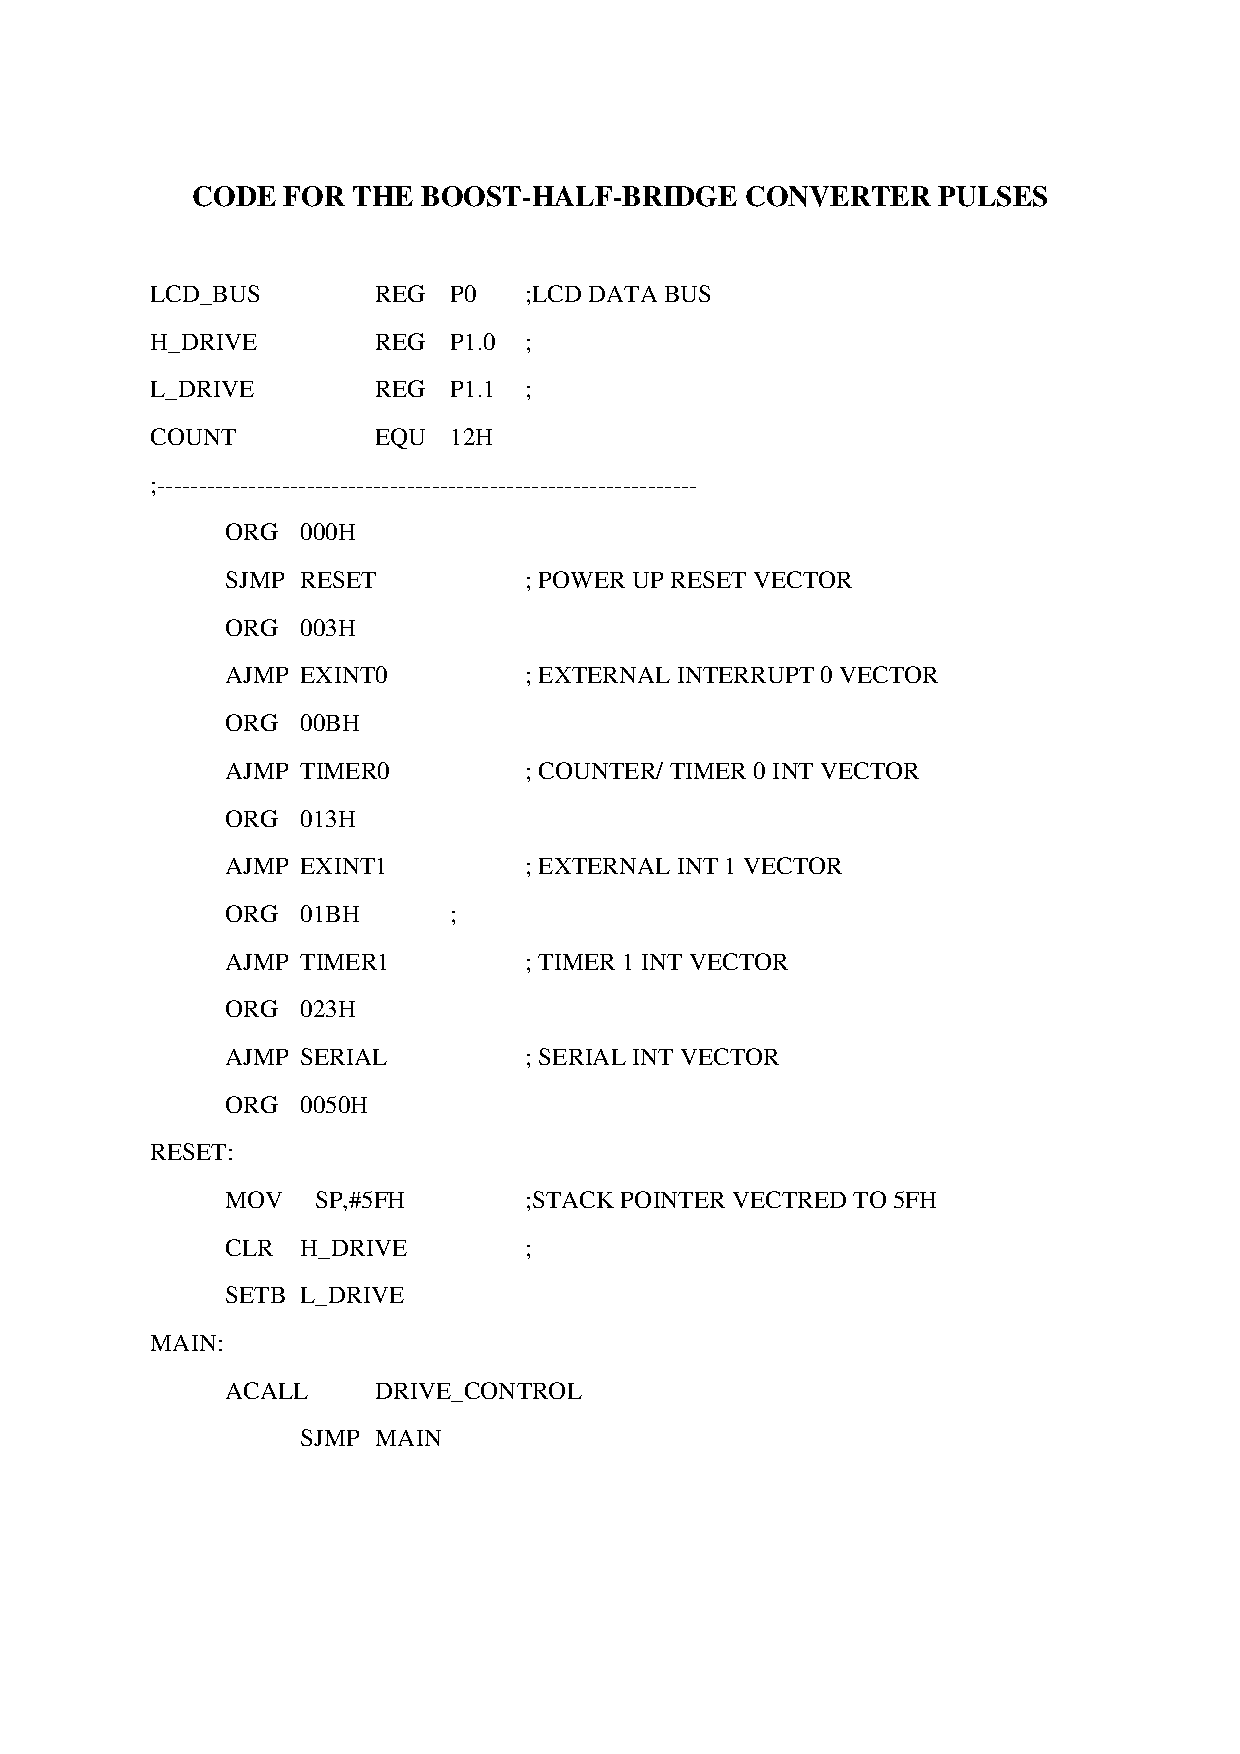
\includepdf[pages=-]{A1.pdf}    % for adding full Paper in PDF
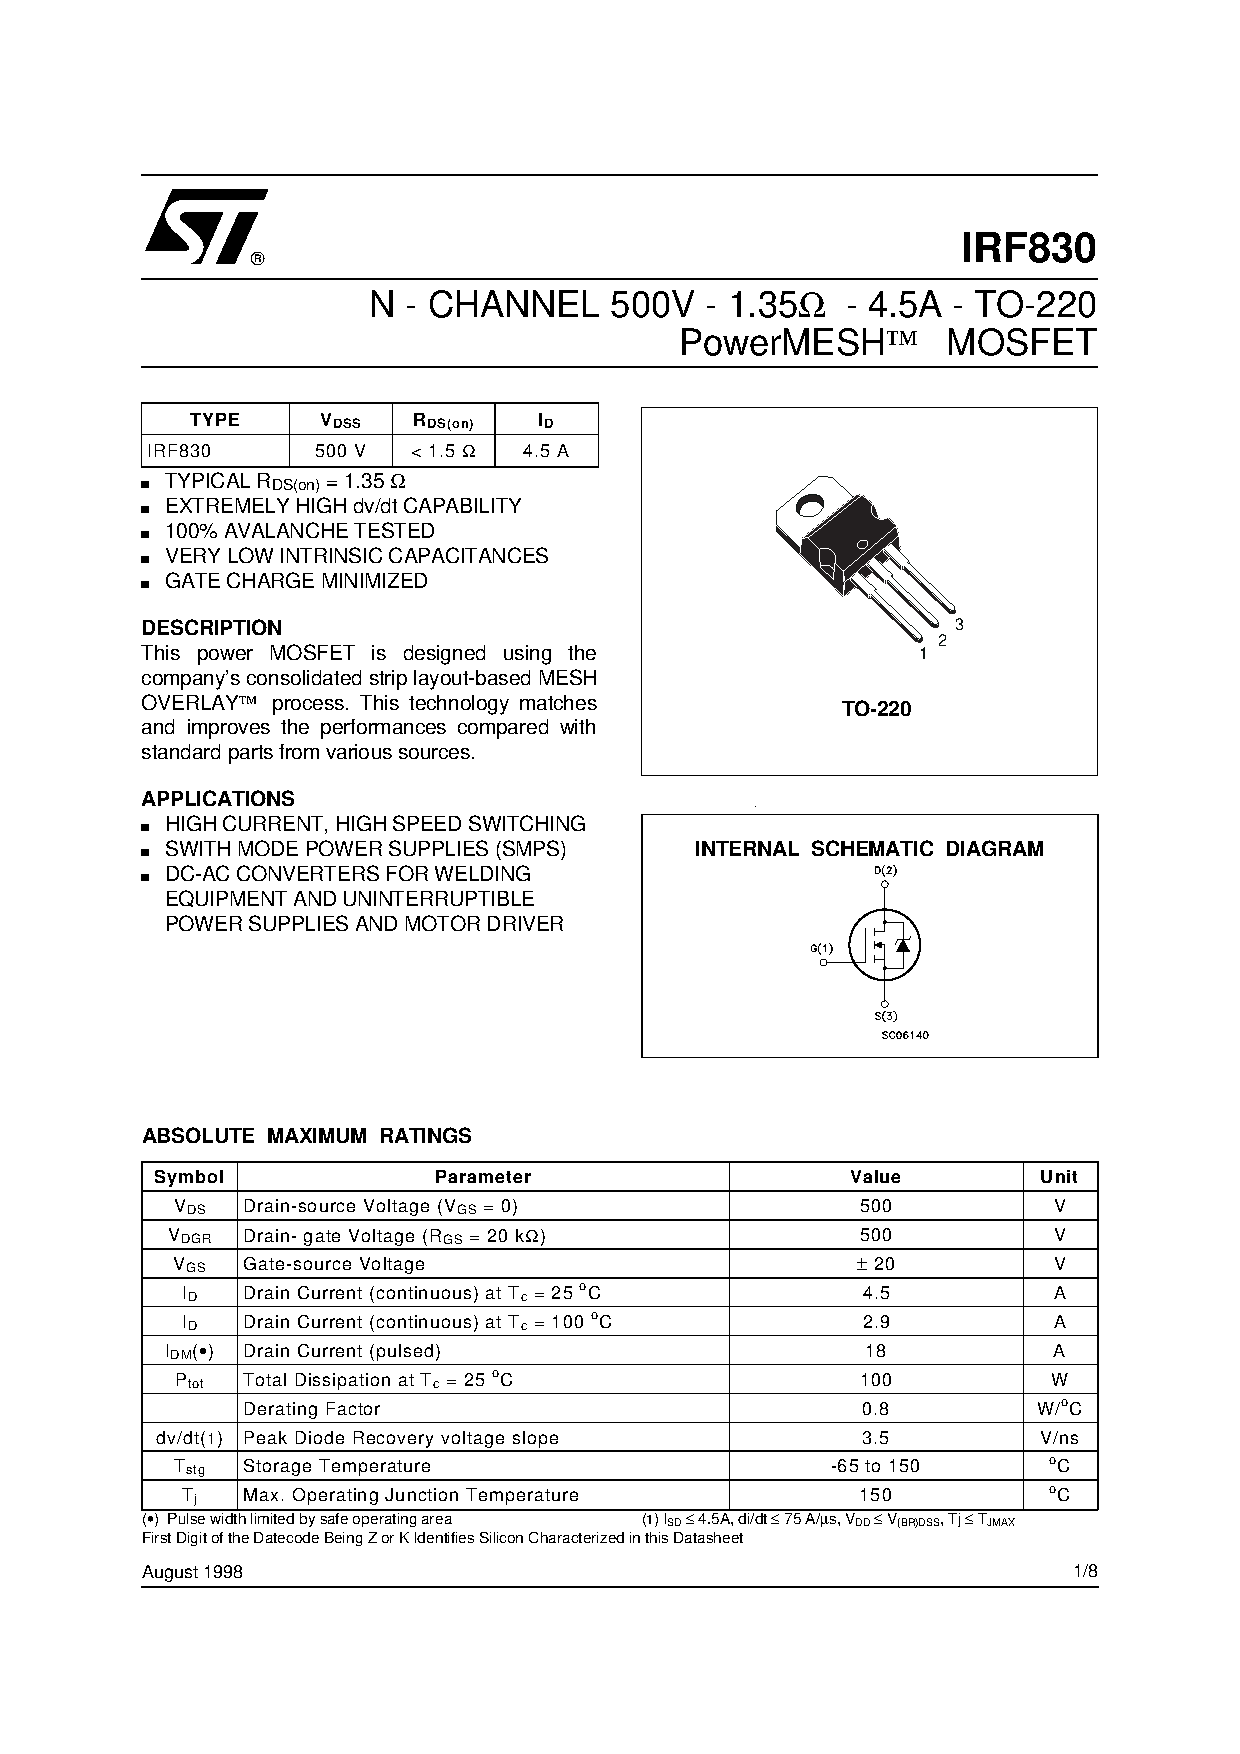
\includepdf[pages=1-3]{IRF830.pdf}    % for adding Pages from 1 to 3 only


%%%%%%%%%%%%%%%%%%%%%%%%%%%%%%%%%%%%%
%%%%%%%%%%%%%%%%%%%%%%%%%%%%%%%%%%%%%
%%%%%%%%%%%%%%%%%%%%%%%%%%%%%%%%%%%%%
%%%%%%%%%%%%%%%%%%%%%%%%%%%%%%%%%%%%%


%%%%%%%%%%%%%%%%%%%%%%%%%%%%%%%%%%%%%
%%%%%%%%%%%%%%%%%%%%%%%%%%%%%%%%%%%%%
%
%   Hi, All 
%
%   Arun Xavier, 
%   Subscribe, Comment at Youtube Channel 
%
%   https://www.youtube.com/c/arunxaviertech
%
%
%   for more  Visit my Page - http://arunxeee.blogspot.in/
%
%%%%%%%%%%%%%%%%%%%%%%%%%%%%%%%%%%%%
%%%%%%%%%%%%%%%%%%%%%%%%%%%%%%%%%%%%

\end{spacing}
\newpage
\thispagestyle{empty}
\vspace*{\fill}
\begin{flushright}

\includegraphics[width=2.5 cm]{VidyaLogo.JPG}\\[.2 cm]
{\Large \bf \rm  Department of \vdept\ Engineering }\\
{\large \rm Vidya Academy of Science \& Technology\\
Thalakkottukara, Thrissur - 680 501\\
({\tt http://www.vidyaacademy.ac.in})}
\end{flushright}

%
\end{document}



%%%%%%	Any Problems Contact me  @  arunxeee.blogspot.com
%%%%%								      aruncx@gmail.com
%%%%%%%%%%%%%%%%
%%%%
%%%%
%%%%%%%%%%%
%%
%